\documentclass[../main.tex]{subfiles}
 
\begin{document}

\section{Thursday}

You luck out. You seem to have had a shift removed from your schedule. In the morning you help a studio responsible for virtual reality content production and distribution. You again find yourself putting VR headsets on people's heads and wiping them down for the next attendee. You're happy to kill downtime during the lulls in the last day's foot traffic by talking to the guy helping to run the booth. He is apparently freelancing for the production company who owns the music videos made for Bono preloaded on each of these headsets. He graduated from UCLA recently with a degree in film; now he's working in a Venice office for the company Within. He seems to have a a few good ideas and you talk at length about Louie C.K.'s new independently produced episodeic content for \textit{Horace and Pete}. You have no idea how he is going to crack into the industry, and you feel starting in VR is possibly a bad move. Unfortunatly, you do't make it over to see the highly praised 360 Google Spotlight Story \textit{Pearl} just a few booths away. While you have been less than impressed with much of the VR stuff that made its way to SIGGRAPH, \textit{Pearl} apparently gets the story part right, and makes use of VR to further the story without relying on the gimmick as so many other booths have done.

With some time before setting off for the beach, you hope to hear a few more technical talks. Unfortunately, when you wander up to the third floor of the Convention Center to pop into Ballroom B for a talk on meshes and fields, you last 5 minutes before you must excuse yourself. The speaker is dreadful and like the Vulcan talk, you cannot get a foothold any point during the presentation. You walk next door to Ballroom C for a presentation titled \textit{Mass Effect: New Earth --- A 4D Holographic Adventure}. The panel doesn't exactly seem to be full of engineers. After a few minutes of marketing baloney with words like "heavy tech" thrown around, you again excuse yourself to look through the bookstore before heading back downstairs. Oh well, you feel like you have gotten a lot out of SIGGRAPH and now shift gears to gathering anyone you can for Huntington beach.

As some of your friends are still finishing their shifts In the final hours of SIGGRAPH, you wonder through Exhibition Hall before all of the vendors close for the day. You check out the a NVIDIA demo where you walk into a trailer hoursing a high powered desktop computer and a HTC Vive setup. You try out an automotive application which allows you to use a controller in your hand to select options which are immediately reflected in a car parked in front of you. What you see in your virtual world is like a large garage, a shiny car on expoxied shop floors. You're encouraged by the gentlemen from Autodesk standing in the room with you to walk over to the car and kneel down inside it. You do, and your mind is just about blown. You can lie down on the floor and look at the underbelly of the car, get up, and walk around it. Your physical controller allows you to point at several orbs in this world to flick between various viewpoints. Because of the cameras positioned in the NVIDEA booth which track your head in high fidelity, you are afforded a VR experience at an entirely different level of immersion that what is offered by Occulus and the Sony Gear (which utilizes an Android phone). You ask some questions and are put off by the overly aggressive sales pitch of the Autodesk marketing guy. He explains that he comes from the automotive industry, and you believe him.

\begin{figure}[h!]
	\centering
	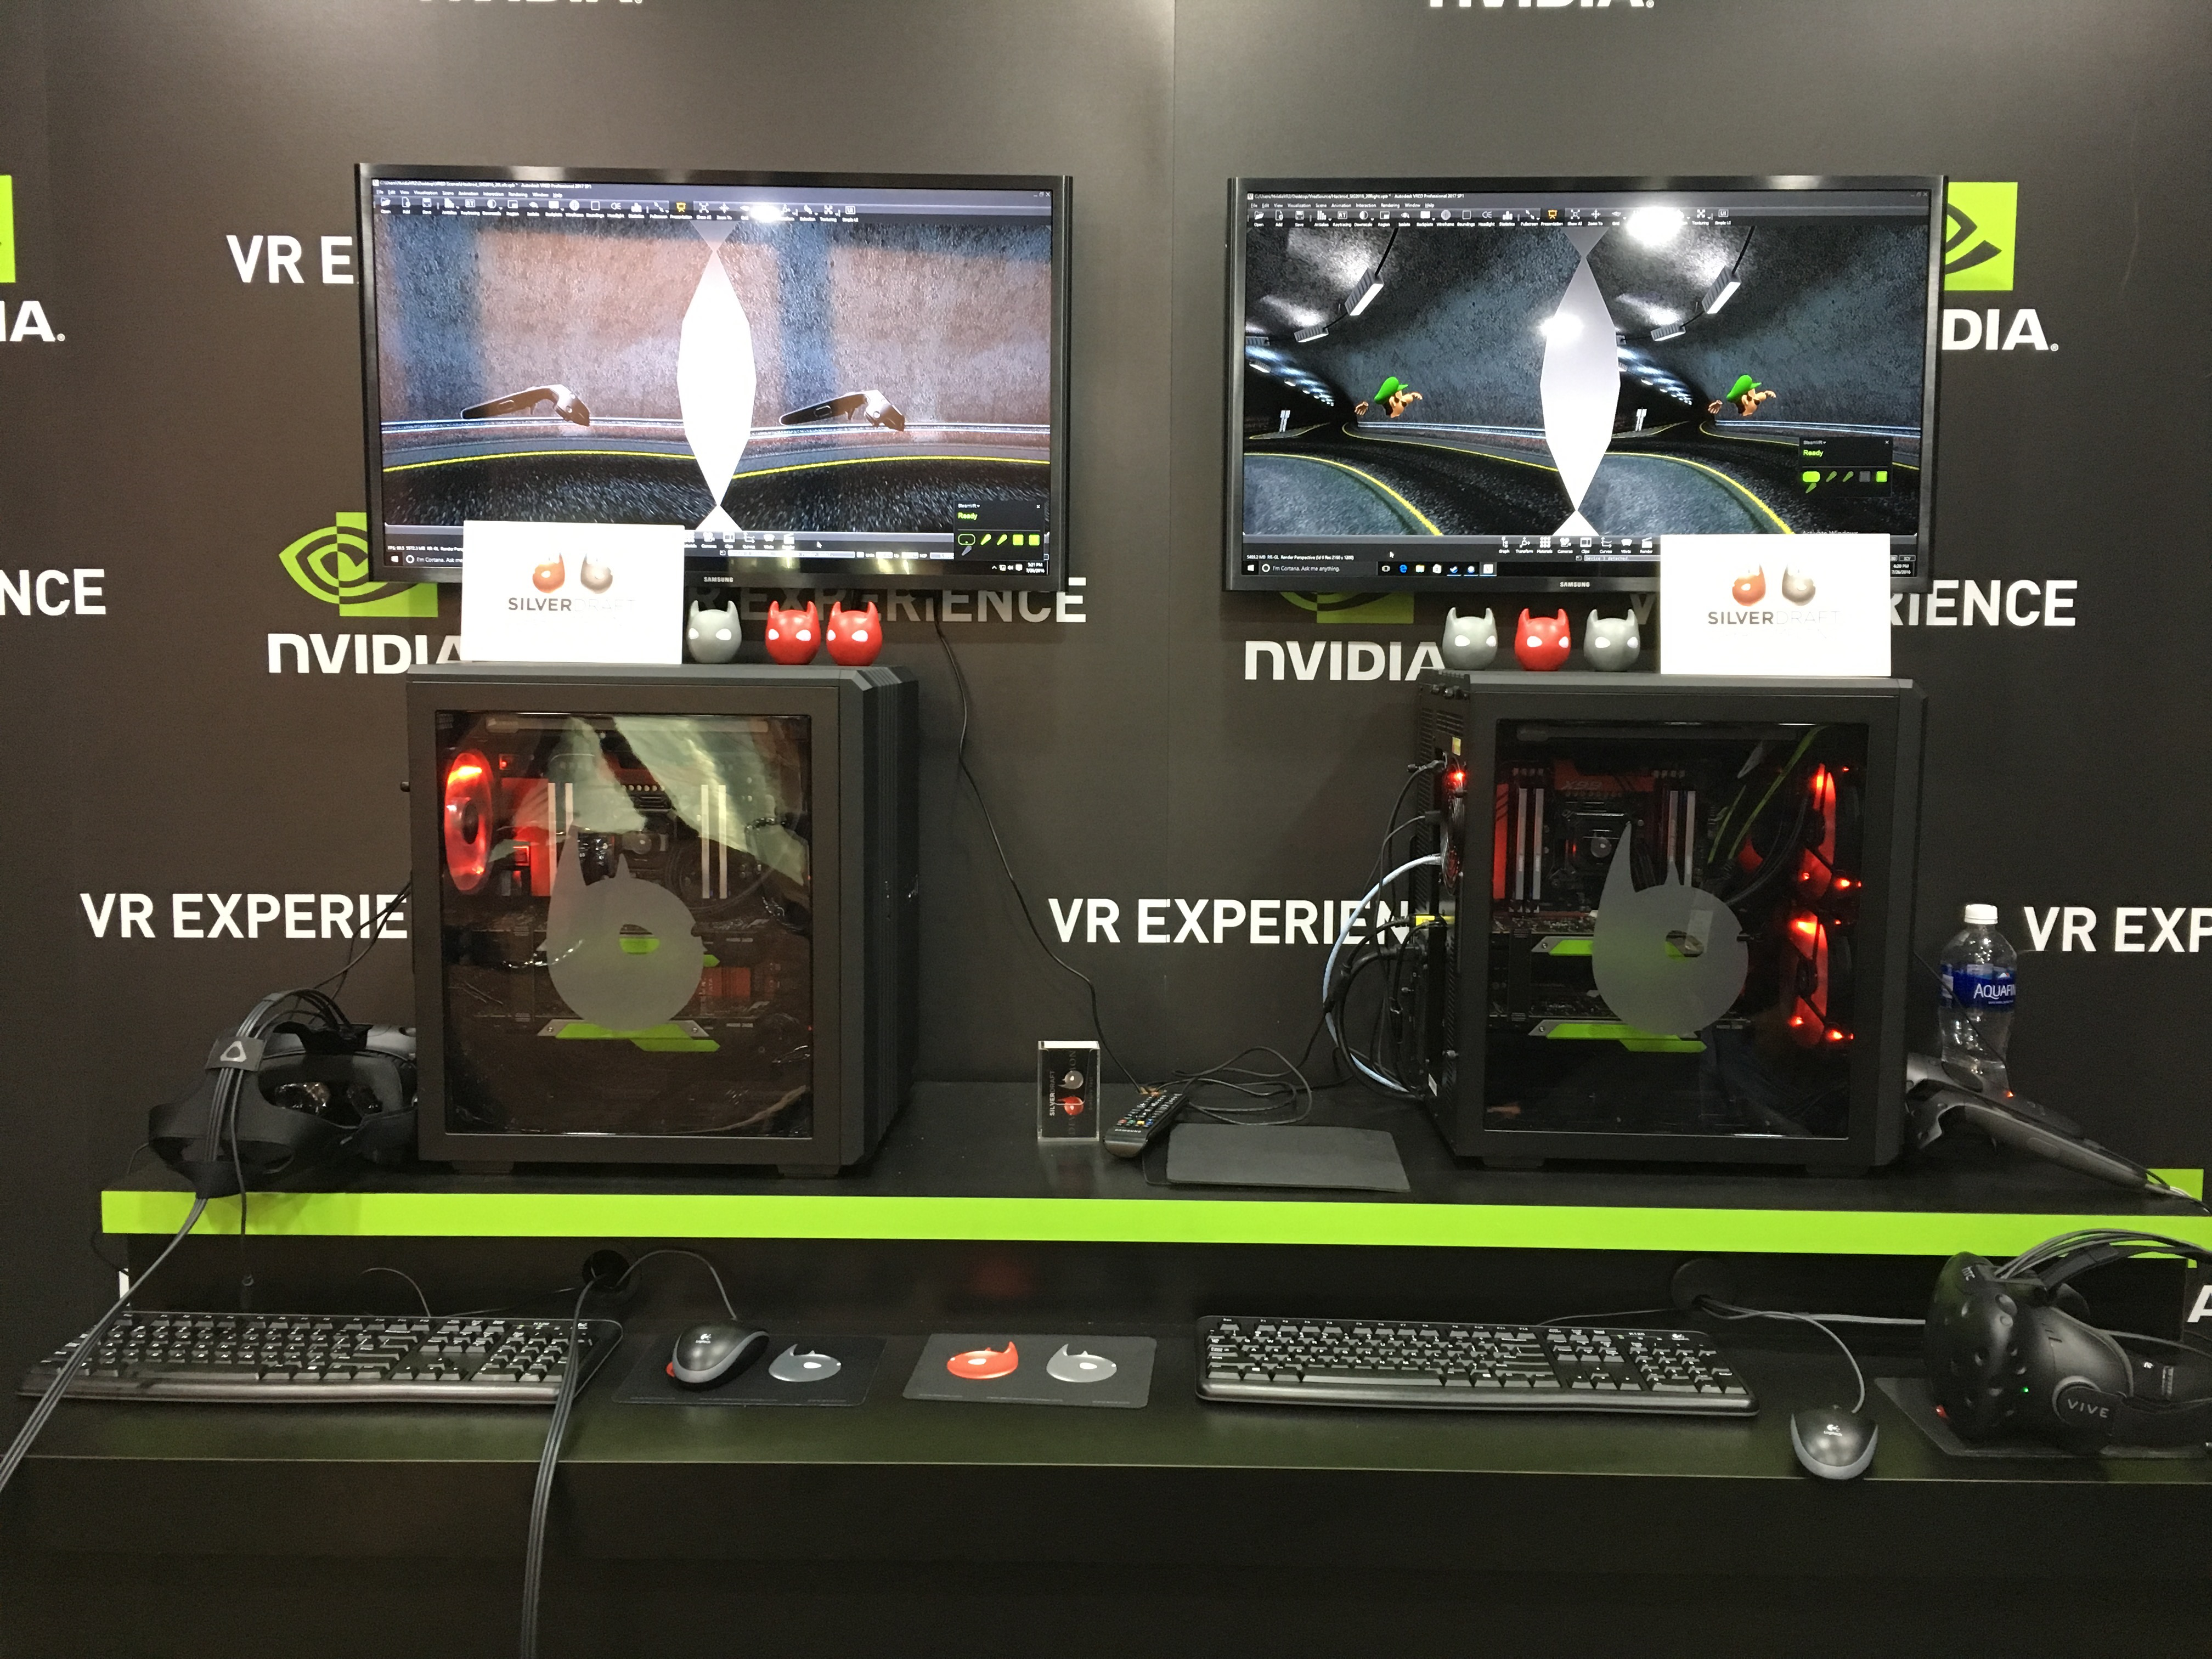
\includegraphics[width=\textwidth]{htc_vive}
	\caption*{The HTC Vive.}
\end{figure}


After collecting people one by one at their hotels, it is Jen, Diede, and another girl named Ambar who pack into a small Uber with you and head to Huntington beach. After a stop at Johnny Rockets, \textit{because 'merica}, you all find a spot in the sand perhaps 20 paces from the water. You haven't been to the beach in a while, and neither has Diede. You have all arrived later than you had hoped, only to experience the golden hour of light descend on you as Jen, Diede, and you take off running into the breaking waves. Perfect. Shivering, you all return to your burgers, pour out Heineken into little red Solo cups, and toast to SIGGRAPH 2016.

\begin{figure}[h!]
	\centering
	
\includegraphics[width=0.6\textwidth]{beach}
	\caption*{Huntington Beach.}
\end{figure}

At some point in the evening, you pose to the group the following question: "What are you really excited about working on when you get back?" Jen describes a vision for an art project that she hopes to complete. You also encourage everyone to go around and share their favorite memories of the past week. You say that yours was seeing the evolution of set design for \textit{Finding Dory}. Stories of college are shared, with Diede at one point describing the fascinating a capella groups at the school he just graduated from in the Netherlands. The night winds down, you all pack back into an Uber and make your way back to a hotel. You all say goodbye and wish each other well, encouraging everyone to stay in touch and not be afraid to reach out. The week is over, but there's no reason you can't keep your world small by keeping tabs on Diede and his work and seeing where Jen and Ambar land in the coming year. You hug, shake Diede's hand, as he half-jokingly insists, and make your way back to your host so that you can pack. You be tired when you wake up early for your flight,  but you did nearly everything you could have hoped to do at your first SIGGRAPH. You learned some new things, received encouragement from people like Philip, made friends, told stories, and came away humbled by the incredible talent of your fellow SVs. You also literally got your feet wet. SIGGRAPH pulls you out of your bubble and reminds you of the beauty of making things and showing them to other people. 

\bigskip

So off you go, to make things.

\end{document}